% Drawing 79/15-12 -- folder 79, batch 15, archive page 290 (PDF page 291).
% Transcription: un pentagone dont tous les sommets sont joints entre eux.
% Kind: hexagon with diagonals (two interlaced triangles). Method 2 (schematic redraw from the facsimile). Status: ok.
% Notes: Light pencil. The outline has six corners (A and B at the top are the two ends of a short top side): A, B, R (right), BR, BL, L (left). Inner strokes: A-BL, A-R, B-L (faint), B-BR, L-BR, and a faint stroke from BL rising to the right that stops on the page short of the right side (at about two thirds of the way up R-BR), drawn so. Every edge is drawn between the same six vertex points. Read so, it is two interlaced triangles (B, L, BR closed; A, R, BL open at the faint stroke); if A and B were one vertex drawn twice it would be a pentagon with its five diagonals, as the transcription says. Redrawn 2026-11-09 (issue 128): to check again. Question settled by a machine pass on the facsimile, 2026-11-12 (page): the outline has six corners (two distinct corners at the ends of the short top side, each the end of its own inner strokes), and the six inner strokes are the sides of the two triangles on alternate corners; a hexagon with two interlaced triangles, as drawn. Not checked by a reader. 2026-11-13, Claude Opus 5.5, overlay check (issue 147): rasterised from its own coordinates over the 400 dpi colour scan (250 ppi native) on a unit grid; the straight edges between the six corners lay 1 to 3 units off the pencil, so the figure is redrawn as the page has it, each of the twelve strokes from where it starts to where it ends on the scan (the sides curve and do not all meet at the corners); laid over the scan again, every stroke lies on its pencil to within about 1 unit. Not compiled (no TeX in the session). Read as before: a hexagon with a short top side, its six inner strokes the sides of two triangles on alternate corners, one of them left open by the faint stroke from the lower left corner that stops short of the right side (the transcription's « pentagone » was corrected on 12 November). Status set to ok.
% Coordinates: 1 unit = 1 mm = 1/100 of the crop width (bbox in page fractions: [0.11, 0.31, 0.31, 0.46]).
% Redrawn by Claude (claude-opus-5-5), issue #73, 2026-11-09; not checked by a human; not compiled (no TeX in the session).
% Checked by Claude (claude-opus-5-5) 2026-11-13 (issue #147): overlaid on the 400 dpi colour facsimile; not compiled (no TeX in the session). Not checked by a human. Status: ok.
% Rights: reproduces part of the work -- behind RENDER_TRANSCRIPTS, never published by itself.
\documentclass[tikz,border=3pt]{standalone}
\usepackage{amsmath,amssymb}
\usetikzlibrary{patterns,arrows.meta}
\tikzset{pencil/.style={black!45}, struck/.style={black!35}, mark/.style={circle,draw,inner sep=1.3pt}, pt/.style={circle,fill,inner sep=0.9pt}, opt/.style={circle,draw,fill=white,inner sep=1.1pt}}
\begin{document}
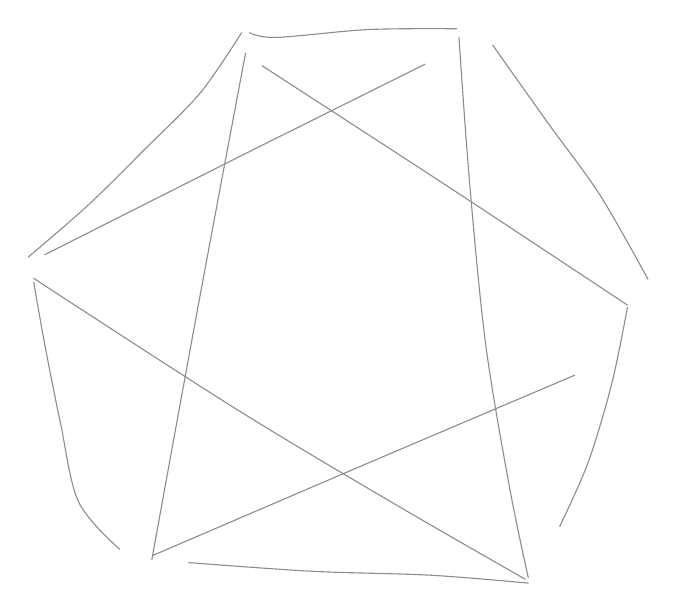
\begin{tikzpicture}[x=1mm,y=1mm,line cap=round,line join=round,font=\scriptsize]
\draw[pencil] plot[smooth, tension=0.55] coordinates {(42,-10.4) (45.4,-11) (57.1,-10) (68.3,-9.9)};
\draw[pencil] plot[smooth, tension=0.55] coordinates {(41,-10.4) (35.7,-18.1) (28.6,-25.3) (21.4,-32.4) (13.9,-38.9)};
\draw[pencil] plot[smooth, tension=0.55] coordinates {(14.6,-42.1) (16,-50) (18,-60) (20.3,-70) (25.5,-76)};
\draw[pencil] plot[smooth, tension=0.55] coordinates {(34.3,-77.7) (50,-78.8) (65,-79.3) (77.4,-80.3)};
\draw[pencil] plot[smooth, tension=0.55] coordinates {(81.4,-73.1) (85,-65) (88,-55) (90,-45.3)};
\draw[pencil] plot[smooth, tension=0.55] coordinates {(72.9,-12) (80,-22) (86.5,-31) (92.6,-41.7)};
\draw[pencil] plot[smooth, tension=0.55] coordinates {(41.5,-13) (35.5,-45) (29.6,-77.3)};
\draw[pencil] plot[smooth, tension=0.55] coordinates {(43.6,-14.6) (67,-29.8) (90,-45)};
\draw[pencil] plot[smooth, tension=0.55] coordinates {(64.3,-14.4) (40,-26.5) (16,-38.6)};
\draw[pencil] plot[smooth, tension=0.55] coordinates {(68.6,-11) (70,-30) (72,-50) (75,-68) (77.4,-79.6)};
\draw[pencil] plot[smooth, tension=0.55] coordinates {(14.6,-41.6) (40,-58) (60,-70) (77,-79.8)};
\draw[pencil] plot[smooth, tension=0.55] coordinates {(29.7,-76.8) (56.5,-65.3) (83.3,-53.9)};
\end{tikzpicture}
\end{document}
